\documentclass[10pt,a4paper,twoside]{book}

%%%%%%%%%%%%%%%%%%%%%%%%%%%%%%%%%%%%%%%%%
% Template Dispense
% Autore: Teo Bonfa (thanks to Teo Bucci)
%%%%%%%%%%%%%%%%%%%%%%%%%%%%%%%%%%%%%%%%%

%---------------------------
% FONTS AND LANGUAGE
%---------------------------

\usepackage[T1]{fontenc}
\usepackage[utf8]{inputenc}
\usepackage[english]{babel}

%---------------------------
% PACKAGES
%---------------------------

\usepackage{dsfont} % for using \mathds{1} characteristic function
\usepackage{amsmath, amssymb, amsthm} % amssymb also loads amsfonts
\usepackage{latexsym}

\usepackage{booktabs}
\usepackage{pgfplots}
\usepackage{tikz}
\usetikzlibrary{
  positioning,
  shapes.misc,
  intersections,
  shapes.symbols,
  patterns,
  fadings,
  shadows.blur,
  decorations.pathreplacing
}
\usepackage{mathdots}
\usepackage{cancel}
\usepackage{color}
\usepackage{siunitx}
\usepackage{array}
\usepackage{multirow}
\usepackage{makecell}
\usepackage{tabularx}
\usepackage{caption}
\captionsetup{belowskip=12pt,aboveskip=4pt}
\usepackage{subcaption}
\usepackage{placeins} % \FloatBarrier
\usepackage{flafter}  % The flafter package ensures that floats don't appear until after they appear in the code.
\usepackage[shortlabels]{enumitem}
\usepackage[italian]{varioref}
\renewcommand{\ref}{\vref}

\newcommand{\quadretti}[3]{ 
\begin{tikzpicture}
\tikzset{normal lines/.style={gray, very thin}} 
\draw[style=normal lines,step=#1] (0,0) grid +(#2,#3); 
\end{tikzpicture}}

% \quadretti{4mm}{160mm}{88mm} % misura lato quadratino, larghezza, altezza del box di quadratini

%---------------------------
% INCLUSIONE FIGURE
%---------------------------

\usepackage{import}
\usepackage{pdfpages}
\usepackage{transparent}
\usepackage{xcolor}
\usepackage{graphicx}
\graphicspath{ {./images/} } % Path relative to the main .tex file
\usepackage{float}

\newcommand{\fg}[3][\relax]{%
  \begin{figure}[H]%[htp]%
    \centering
    \captionsetup{width=0.7\textwidth}
      \includegraphics[width = #2\textwidth]{#3}%
      \ifx\relax#1\else\caption{#1}\fi
      \label{#3}
  \end{figure}%
  \FloatBarrier%
}
%\usepackage[labelformat=empty]{caption}

%\captionsetup{belowskip=0pt,aboveskip=0pt}

\let\origtopsep\topsep
\newenvironment{hfigure}[1][\origtopsep]{\begingroup\captionsetup{belowskip=0pt,aboveskip=2pt}
\setlength{\topsep}{#1}\begin{center}}
{\end{center}\endgroup}

%---------------------------
% PARAGRAPHS AND LINES
%---------------------------

\usepackage[none]{hyphenat} % no hyphenation

\emergencystretch 3em % to prevent the text from going beyond margins

\usepackage[skip=0.2\baselineskip+2pt]{parskip}

% \renewcommand{\baselinestretch}{1.5} % line spacing

%---------------------------
% HEADERS AND FOOTERS
%---------------------------

\usepackage{fancyhdr}

\fancypagestyle{toc}{%
\fancyhf{}%
\fancyfoot[C]{\thepage}%
\renewcommand{\headrulewidth}{0pt}%
\renewcommand{\footrulewidth}{0pt}
}

\fancypagestyle{fancy}{%
\fancyhf{}%
\fancyhead[RE]{\nouppercase{\leftmark}}%
\fancyhead[LO]{\nouppercase{\rightmark}}%
\fancyhead[LE,RO]{\thepage}%
\renewcommand{\footrulewidth}{0pt}%
\renewcommand{\headrulewidth}{0.4pt}
}

% Removes the header from odd empty pages at the end of chapters
\makeatletter
\renewcommand{\cleardoublepage}{
\clearpage\ifodd\c@page\else
\hbox{}
\vspace*{\fill}
\thispagestyle{empty}
\newpage
\fi}

\usepackage{nonumonpart}

%---------------------------
% CUSTOM
%---------------------------

\usepackage{xspace}
\newcommand{\latex}{\LaTeX\xspace}
\newcommand{\tex}{\TeX\xspace}

\newcommand{\Tau}{\mathcal{T}}
\newcommand{\Ind}{\mathds{1}} % indicatrice

\newcommand{\transpose}{^{\mathrm{T}}}
\newcommand{\complementary}{^{\mathrm{C}}} % alternative ^{\mathrm{C}} ^{\mathrm{c}} ^{\mathsf{c}}
\newcommand{\degree}{^\circ\text{C}} % simbolo gradi

\newcommand{\notimplies}{\mathrel{{\ooalign{\hidewidth$\not\phantom{=}$\hidewidth\cr$\implies$}}}}
\newcommand{\questeq}{\overset{?}{=}} % è vero che?

\newcommand{\indep}{\perp \!\!\! \perp} % indipendenza
\newcommand{\iid}{\stackrel{\mathrm{iid}}{\sim}}
\newcommand{\event}[1]{\emph{``#1''}} % evento

% variazioni del simbolo "="
\newcommand{\iideq}{\overset{\text{\tiny iid}}{=}}
\newcommand{\ideq}{\overset{\text{\tiny id}}{=}}
\newcommand{\indepeq}{\overset{\perp \!\!\! \perp}{=}}

\newcommand{\boxedText}[1]{\noindent\fbox{\parbox{\textwidth}{#1}}}

\renewcommand{\emptyset}{\varnothing}
\renewcommand{\tilde}{\widetilde}
\renewcommand{\hat}{\widehat}

\DeclareMathOperator{\sgn}{sgn}
\DeclareMathOperator{\Var}{Var}
\DeclareMathOperator{\Cov}{Cov}
\DeclareMathOperator*{\rank}{rank}
\DeclareMathOperator*{\eig}{eig}
\DeclareMathOperator{\tr}{tr}
%\DeclareMathOperator{\Grad}{grad}
%\DeclareMathOperator{\Div}{div}
\DeclareMathOperator{\Span}{span}
\let\Re\undefined  % redefine \Re
\DeclareMathOperator{\Re}{Re}
\let\Im\undefined  % redefine \Im
\DeclareMathOperator{\Im}{Im}
\DeclareMathOperator{\Ker}{Ker}
\DeclareMathOperator*{\argmin}{arg\,min}
\DeclareMathOperator*{\argmax}{arg\,max}
\DeclareMathOperator*{\esssup}{ess\ sup}
\DeclareMathOperator*{\essinf}{ess\ inf}
\DeclareMathOperator*{\supp}{supp}

\newcommand{\eps}{\varepsilon}
\renewcommand{\theta}{\vartheta}

% Per scrivere il numero e la data della lezione


\usepackage{mathtools} % Serve per i comandi dopo
%\DeclarePairedDelimiter{\abs}{\lvert}{\rvert} % absolute value
%\DeclarePairedDelimiter{\sca}{\langle}{\rangle} % scalar product
%\DeclarePairedDelimiter{\norm}{\lVert}{\rVert} % norm
\newcommand{\abs}[1]{\left\lvert #1 \right\rvert}
\newcommand{\norm}[1]{\left\lVert #1 \right\rVert}
\newcommand{\sca}[1]{\left\langle #1 \right\rangle}
\newcommand{\parteInf}[1]{\left\lfloor #1 \right\rfloor}
\newcommand{\parteSup}[1]{\left\lceil #1 \right\rceil}

\newcommand{\gr}[1]{\left\{ #1 \right\}}
\newcommand{\qu}[1]{\left[ #1 \right]}
\newcommand{\td}[1]{\left(#1 \right)}

\newcommand{\equalexpl}[1]{%
  \underset{\substack{\uparrow\\\vspace{-2em}\mathrlap{\text{#1}}}}{\hspace{0.3em}=}
}
\newcommand{\leqexpl}[1]{%
  \underset{\substack{\uparrow\\\vspace{-2em}\mathrlap{\text{#1}}}}{\hspace{0.3em}\leq}
}
\newcommand{\arrowlexpl}[1]{%
  \underset{\substack{\uparrow\\\vspace{-2em}\mathrlap{\text{#1}}}}{\hspace{0.3em}$\Rightarrow$}
}

% Bold
\renewcommand{\AA}{\mathbb A}
\newcommand{\BB}{\mathbb{B}}
\newcommand{\CC}{\mathbb{C}}
\newcommand{\DD}{\mathbb{D}}
\newcommand{\EE}{\mathbb{E}}
\newcommand{\FF}{\mathbb{F}}
\newcommand{\GG}{\mathbb{G}}
\newcommand{\HH}{\mathbb{H}}
\newcommand{\II}{\mathbb{I}}
\newcommand{\JJ}{\mathbb{J}}
\newcommand{\KK}{\mathbb{K}}
\newcommand{\LL}{\mathbb{L}}
\newcommand{\MM}{\mathbb{M}}
\newcommand{\NN}{\mathbb{N}}
\newcommand{\OO}{\mathbb{O}}
\newcommand{\PP}{\mathbb{P}}
\newcommand{\QQ}{\mathbb{Q}}
\newcommand{\RR}{\mathbb{R}}
\renewcommand{\SS}{\mathbb S}
\newcommand{\TT}{\mathbb{T}}
\newcommand{\UU}{\mathbb{U}}
\newcommand{\VV}{\mathbb{V}}
\newcommand{\WW}{\mathbb{W}}
\newcommand{\XX}{\mathbb{X}}
\newcommand{\YY}{\mathbb{Y}}
\newcommand{\ZZ}{\mathbb{Z}}

% Calligraphic 
\usepackage{euscript} % accedi a Euler usando \EuScript{}
\usepackage[cal=dutchcal,calscaled=.97]{mathalfa} % default calligraphic font, accedi con \mathcal{}
\DeclareMathAlphabet{\modern}{OMS}{zplm}{m}{n} % accedi al calligrafico predefinito (computer modern roman) usando \modern{}

\DeclareMathAlphabet{\mathrsfso}{U}{rsfso}{m}{n}
\newcommand{\rsf}{\mathrsfso}

\DeclareFontFamily{U}{BOONDOX-calo}{\skewchar\font=45}
\DeclareFontShape{U}{BOONDOX-calo}{m}{n}{
  <-> s*[1.05] BOONDOX-r-calo}{}
\DeclareMathAlphabet{\mathcalboondox}{U}{BOONDOX-calo}{m}{n}
\newcommand{\bondox}{\mathcalboondox}

% Calligrafico predefinito (Computer Modern Roman)
\newcommand{\Ac}{\modern{A}}
\newcommand{\Bc}{\modern{B}}
\newcommand{\Cc}{\modern{C}} % for C^0 
\newcommand{\Dc}{\modern{D}}
\newcommand{\Ec}{\modern{E}} % for epsilon in the proofs
\newcommand{\Fc}{\modern{F}}
\newcommand{\Gc}{\modern{G}}
\newcommand{\Hc}{\modern{H}}
\newcommand{\Ic}{\modern{I}}
\newcommand{\Jc}{\modern{J}}
\newcommand{\Kc}{\modern{K}}
\newcommand{\Lc}{\modern{L}}
\newcommand{\Mc}{\modern{M}}
\newcommand{\Nc}{\modern{N}}
\newcommand{\Oc}{\modern{O}}
\newcommand{\Pc}{\modern{P}}
\newcommand{\Qc}{\modern{Q}}
\newcommand{\Rc}{\modern{R}}
\newcommand{\Sc}{\modern{S}}
\newcommand{\Tc}{\modern{T}}
\newcommand{\Uc}{\modern{U}}
\newcommand{\Vc}{\modern{V}}
\newcommand{\Wc}{\modern{W}}
\newcommand{\Xc}{\modern{X}}
\newcommand{\Yc}{\modern{Y}}
\newcommand{\Zc}{\modern{Z}}

% Calligrafico EUler
\newcommand{\Aeu}{\EuScript{A}}
\newcommand{\Beu}{\EuScript{B}}
\newcommand{\Ceu}{\EuScript{C}}
\newcommand{\Deu}{\EuScript{D}}
\newcommand{\Eeu}{\EuScript{E}}
\newcommand{\Feu}{\EuScript{F}}
\newcommand{\Geu}{\EuScript{G}}
\newcommand{\Heu}{\EuScript{H}}
\newcommand{\Ieu}{\EuScript{I}}
\newcommand{\Jeu}{\EuScript{J}}
\newcommand{\Keu}{\EuScript{K}}
\newcommand{\Leu}{\EuScript{L}}
\newcommand{\Meu}{\EuScript{M}}
\newcommand{\Neu}{\EuScript{N}}
\newcommand{\Oeu}{\EuScript{O}}
\newcommand{\Peu}{\EuScript{P}} % for the power set
\newcommand{\Qeu}{\EuScript{Q}}
\newcommand{\Reu}{\EuScript{R}}
\newcommand{\Seu}{\EuScript{S}}
\newcommand{\Teu}{\EuScript{T}} % for topological stuff
\newcommand{\Ueu}{\EuScript{U}}
\newcommand{\Veu}{\EuScript{V}}
\newcommand{\Weu}{\EuScript{W}}
\newcommand{\Xeu}{\EuScript{X}}
\newcommand{\Yeu}{\EuScript{Y}}
\newcommand{\Zeu}{\EuScript{Z}}

% Calligrafico dutchcal
\newcommand{\Adu}{\mathcal{A}}
\newcommand{\Bdu}{\mathcal{B}} % for Borel stuff
\newcommand{\Cdu}{\mathcal{C}}
\newcommand{\Ddu}{\mathcal{D}}
\newcommand{\Edu}{\mathcal{E}}
\newcommand{\Fdu}{\mathcal{F}}
\newcommand{\Gdu}{\mathcal{G}}
\newcommand{\Hdu}{\mathcal{H}}
\newcommand{\Idu}{\mathcal{I}}
\newcommand{\Jdu}{\mathcal{J}}
\newcommand{\Kdu}{\mathcal{K}}
\newcommand{\Ldu}{\mathcal{L}}
\newcommand{\Mdu}{\mathcal{M}} % for sigma-algebras
\newcommand{\Ndu}{\mathcal{N}}
\newcommand{\Odu}{\mathcal{O}}
\newcommand{\Pdu}{\mathcal{P}}
\newcommand{\Qdu}{\mathcal{Q}}
\newcommand{\Rdu}{\mathcal{R}}
\newcommand{\Sdu}{\mathcal{S}}
\newcommand{\Tdu}{\mathcal{T}}
\newcommand{\Udu}{\mathcal{U}}
\newcommand{\Vdu}{\mathcal{V}}
\newcommand{\Wdu}{\mathcal{W}}
\newcommand{\Xdu}{\mathcal{X}}
\newcommand{\Ydu}{\mathcal{Y}}
\newcommand{\Zdu}{\mathcal{Z}}

% Bold Big Vector
\newcommand{\Av}{\mathbf{A}}
\newcommand{\Bv}{\mathbf{B}}
\newcommand{\Cv}{\mathbf{C}}
\newcommand{\Dv}{\mathbf{D}}
\newcommand{\Ev}{\mathbf{E}}
\newcommand{\Fv}{\mathbf{F}}
\newcommand{\Gv}{\mathbf{G}}
\newcommand{\Hv}{\mathbf{H}}
\newcommand{\Iv}{\mathbf{I}}
\newcommand{\Jv}{\mathbf{J}}
\newcommand{\Kv}{\mathbf{K}}
\newcommand{\Lv}{\mathbf{L}}
\newcommand{\Mv}{\mathbf{M}}
\newcommand{\Nv}{\mathbf{N}}
\newcommand{\Ov}{\mathbf{O}}
\newcommand{\Pv}{\mathbf{P}}
\newcommand{\Qv}{\mathbf{Q}}
\newcommand{\Rv}{\mathbf{R}}
\newcommand{\Sv}{\mathbf{S}}
\newcommand{\Tv}{\mathbf{T}}
\newcommand{\Uv}{\mathbf{U}}
\newcommand{\Vv}{\mathbf{V}}
\newcommand{\Wv}{\mathbf{W}}
\newcommand{\Xv}{\mathbf{X}}
\newcommand{\Yv}{\mathbf{Y}}
\newcommand{\Zv}{\mathbf{Z}}

% Bold Little Vector
\newcommand{\av}{\mathbf{a}}
\newcommand{\bv}{\mathbf{b}}
\newcommand{\cv}{\mathbf{c}}
\newcommand{\dv}{\mathbf{d}}
\newcommand{\ev}{\mathbf{e}}
\newcommand{\fv}{\mathbf{f}}
\newcommand{\gv}{\mathbf{g}}
\newcommand{\hv}{\mathbf{h}}
\newcommand{\iv}{\mathbf{i}}
\newcommand{\jv}{\mathbf{j}}
\newcommand{\kv}{\mathbf{k}}
\newcommand{\lv}{\mathbf{l}}
\newcommand{\mv}{\mathbf{m}}
\newcommand{\nv}{\mathbf{n}}
\newcommand{\ov}{\mathbf{o}}
\newcommand{\pv}{\mathbf{p}}
\newcommand{\qv}{\mathbf{q}}
\newcommand{\rv}{\mathbf{r}}
\newcommand{\sv}{\mathbf{s}}
\newcommand{\tv}{\mathbf{t}}
\newcommand{\uv}{\mathbf{u}}
\newcommand{\vv}{\mathbf{v}}
\newcommand{\wv}{\mathbf{w}}
\newcommand{\xv}{\mathbf{x}}
\newcommand{\yv}{\mathbf{y}}
\newcommand{\zv}{\mathbf{z}}

% differenziale
\newcommand{\dspace}{\ } % \, aggiunge un piccolo spazio
\newcommand{\de}{\mathrm{d}}
\newcommand{\dx}{\dspace \de x}
\newcommand{\dy}{\dspace \de y}
\newcommand{\dt}{\dspace \de t}
\newcommand{\dS}{\dspace \de S}
\newcommand{\ds}{\dspace \de s}
\newcommand{\dz}{\dspace \de z}
\newcommand{\dw}{\dspace \de w}
\newcommand{\du}{\dspace \de u}
\newcommand{\dvv}{\dspace \de v}
\newcommand{\db}{\dspace \de b}
\newcommand{\dteta}{\dspace \de \vartheta}
\newcommand{\dxi}{\dspace \de \xi}
\newcommand{\dxy}{\dspace \de x \de y}
\newcommand{\duv}{\dspace \de u \de v}
\newcommand{\dst}{\dspace \de s \de t}
\newcommand{\dP}{\dspace \de P}
\newcommand{\dPP}{\dspace \de \PP}
\newcommand{\dsig}{\dspace \de \sigma}
\newcommand{\dth}{\dspace \de \theta}
\newcommand{\deta}{\dspace \de \eta}
\newcommand{\dph}{\dspace \de \varphi}
\newcommand{\dxv}{\dspace \de \mathbf{x}}
\newcommand{\dSx}{\dspace \de \text{S}(x)}

\newcommand{\Grad}{\nabla}
\newcommand{\Div}{\mathrm{div}}
\newcommand{\Lap}{\Delta}
% \newcommand{\Dalem}{\Box} per l'eq delle onde?

\newcommand{\SDP}{(\Omega,\Ac,\PP)} % spazio di probabilità
\newcommand{\Omegaa}{\overline{\Omega}} % chiusura
\newcommand{\Cz}{\Cc^0}
\newcommand{\Cu}{\Cc^1}
\newcommand{\Cd}{\Cc^2}
\newcommand{\Lu}{\mathcal{L}^1}
\newcommand{\ld}{\ell^2}
\newcommand{\frp}{\partial_pQ_T}

\newcommand{\hod}[1]{^{\scriptscriptstyle\mathrm{#1}}} % per le derivate con exp romano

%\newcommand{\Log}{\text{Log}}

% spaziature https://tex.stackexchange.com/questions/438612/space-between-exists-and-forall
% questo aggiunge un piccolo spazio dopo \forall
\let\oldforall\forall
\renewcommand{\forall}{\oldforall \, }
% questo aggiunge un piccolo spazio dopo \exists
\let\oldexist\exists
\renewcommand{\exists}{\oldexist \: }
% questo aggiunge un comando \existsu per l'esiste ed è unico
\newcommand\existu{\oldexist! \: }

%---------------------------
% APPENDICE
%---------------------------

\usepackage[title,titletoc]{appendix}

%---------------------------
% THEOREMS
%---------------------------

\definecolor{grey245}{RGB}{245,245,245}

\newtheoremstyle{blacknumbox} % Theorem style name
{0pt}% Space above
{0pt}% Space below
{\normalfont}% Body font
{}% Indent amount
{\bf\scshape}% Theorem head font --- {\small\bf}
{.\;}% Punctuation after theorem head
{0.25em}% Space after theorem head
{\small\thmname{#1}\nobreakspace\thmnumber{\@ifnotempty{#1}{}\@upn{#2}}% Theorem text (e.g. Theorem 2.1)
%{\small\thmname{#1}% Theorem text (e.g. Theorem)
\thmnote{\nobreakspace\the\thm@notefont\normalfont\bfseries---\nobreakspace#3}}% Optional theorem note

\newtheoremstyle{unnumbered} % Theorem style name
{0pt}% Space above
{0pt}% Space below
{\normalfont}% Body font
{}% Indent amount
{\bf\scshape}% Theorem head font --- {\small\bf}
{.\;}% Punctuation after theorem head
{0.25em}% Space after theorem head
{\small\thmname{#1}\thmnumber{\@ifnotempty{#1}{}\@upn{#2}}% Theorem text (e.g. Theorem 2.1)
%{\small\thmname{#1}% Theorem text (e.g. Theorem)
\thmnote{\nobreakspace\the\thm@notefont\normalfont\bfseries---\nobreakspace#3}}% Optional theorem note

\newtheoremstyle{demo} % Theorem style name
{0pt}% Space above
{0pt}% Space below
{\normalfont}% Body font
{}% Indent amount
{\bf\scshape}% Theorem head font --- {\small\bf}
{.\;}% Punctuation after theorem head
{0.25em}% Space after theorem head
{\small\thmname{#1}\thmnumber{\@ifnotempty{#1}{}\@upn{#2}}% Theorem text (e.g. Theorem 2.1)
%{\small\thmname{#1}% Theorem text (e.g. Theorem)
\thmnote{\nobreakspace\the\thm@notefont\normalfont\bfseries\footnotesize{(#3)}}}% Optional theorem note

\newcounter{dummy}
\numberwithin{dummy}{chapter}

\newcounter{dummyNOT}
\numberwithin{dummyNOT}{chapter}

\theoremstyle{blacknumbox}
\newtheorem{theoremT}[dummy]{Theorem}
\newtheorem{corollaryT}[dummy]{Corollary}
\newtheorem{lemmaT}[dummy]{Lemma}
\newtheorem{propositionT}[dummy]{Proposition}

% Per gli unnumbered tolgo il \nobreakspace subito dopo {\small\thmname{#1} perché altrimenti c'è uno spazio tra Teorema e il ".", lo spazio lo voglio solo se sono numerati per distanziare Teorema e "(2.1)"
\theoremstyle{unnumbered}
\newtheorem*{remarkT}{Remark}
\newtheorem*{exampleT}{Example}
\newtheorem*{propertyT}{Property}
\newtheorem*{homeworkT}{Homework}
\newtheorem*{hintT}{Subtleties}
\newtheorem*{definitionT}{Definition}
\newtheorem*{exerciseT}{Exercise}

\theoremstyle{demo}
\newtheorem*{proofT}{Proof}

\RequirePackage[framemethod=default]{mdframed} % Required for creating the theorem, definition, exercise and corollary boxes

% orange box
\newmdenv[skipabove=7pt,
skipbelow=4pt,
rightline=true,
leftline=true,
topline=true,
bottomline=true,
linecolor=orange,
backgroundcolor=orange!0,
innerleftmargin=5pt,
innerrightmargin=5pt,
innertopmargin=5pt,
leftmargin=0cm,
rightmargin=0cm,
linewidth=1pt,
innerbottommargin=5pt]{oBox}

% green box
\newmdenv[skipabove=7pt,
skipbelow=4pt,
rightline=true,
leftline=true,
topline=true,
bottomline=true,
linecolor=green,
backgroundcolor=green!0,
innerleftmargin=5pt,
innerrightmargin=5pt,
innertopmargin=5pt,
leftmargin=0cm,
rightmargin=0cm,
linewidth=1pt,
innerbottommargin=5pt]{gBox}

% blue box
\newmdenv[skipabove=7pt,
skipbelow=4pt,
rightline=true,
leftline=true,
topline=true,
bottomline=true,
linecolor=blue,
backgroundcolor=blue!0,
innerleftmargin=5pt,
innerrightmargin=5pt,
innertopmargin=5pt,
leftmargin=0cm,
rightmargin=0cm,
linewidth=1pt,
innerbottommargin=5pt]{bBox}

% purple box
\newmdenv[skipabove=7pt,
skipbelow=4pt,
rightline=true,
leftline=true,
topline=true,
bottomline=true,
linecolor=purple,
backgroundcolor=purple!0,
innerleftmargin=5pt,
innerrightmargin=5pt,
innertopmargin=5pt,
leftmargin=0cm,
rightmargin=0cm,
linewidth=1pt,
innerbottommargin=5pt]{pBox}

% hunter green box
\definecolor{huntergreen}{rgb}{0.21, 0.37, 0.23}
\newmdenv[skipabove=7pt,
skipbelow=4pt,
rightline=true,
leftline=true,
topline=true,
bottomline=true,
linecolor=huntergreen,
backgroundcolor=huntergreen!0,
innerleftmargin=5pt,
innerrightmargin=5pt,
innertopmargin=5pt,
leftmargin=0cm,
rightmargin=0cm,
linewidth=1pt,
innerbottommargin=5pt]{hBox}

% lavender (floral) box
\definecolor{lavender(floral)}{rgb}{0.71, 0.49, 0.86}
\newmdenv[skipabove=7pt,
skipbelow=4pt,
rightline=true,
leftline=true,
topline=true,
bottomline=true,
linecolor=lavender(floral),
backgroundcolor=lavender(floral)!0,
innerleftmargin=5pt,
innerrightmargin=5pt,
innertopmargin=5pt,
leftmargin=0cm,
rightmargin=0cm,
linewidth=1pt,
innerbottommargin=5pt]{lBox}

% air force blue box
\definecolor{airforceblue}{rgb}{0.36, 0.54, 0.66}
\newmdenv[skipabove=7pt,
skipbelow=4pt,
rightline=true,
leftline=true,
topline=true,
bottomline=true,
linecolor=airforceblue,
backgroundcolor=airforceblue!0,
innerleftmargin=5pt,
innerrightmargin=5pt,
innertopmargin=5pt,
leftmargin=0cm,
rightmargin=0cm,
linewidth=1pt,
innerbottommargin=5pt]{aBox}

% teal box
\newmdenv[skipabove=7pt,
skipbelow=4pt,
rightline=true,
leftline=true,
topline=true,
bottomline=true,
linecolor=teal,
backgroundcolor=teal!0,
innerleftmargin=5pt,
innerrightmargin=5pt,
innertopmargin=5pt,
leftmargin=0cm,
rightmargin=0cm,
linewidth=1pt,
innerbottommargin=5pt]{tBox}

% gold box
\definecolor{satinsheengold}{rgb}{0.8, 0.63, 0.21}
\newmdenv[skipabove=7pt,
skipbelow=4pt,
rightline=true,
leftline=true,
topline=true,
bottomline=true,
linecolor=satinsheengold,
backgroundcolor=satinsheengold!0,
innerleftmargin=5pt,
innerrightmargin=5pt,
innertopmargin=5pt,
leftmargin=0cm,
rightmargin=0cm,
linewidth=1pt,
innerbottommargin=5pt]{sBox}

% atomic tangerine box
\definecolor{atomictangerine}{rgb}{1.0, 0.6, 0.4}
\newmdenv[skipabove=7pt,
skipbelow=4pt,
rightline=true,
leftline=true,
topline=true,
bottomline=true,
linecolor=atomictangerine,
backgroundcolor=atomictangerine!0,
innerleftmargin=5pt,
innerrightmargin=5pt,
innertopmargin=5pt,
leftmargin=0cm,
rightmargin=0cm,
linewidth=1pt,
innerbottommargin=5pt]{atBox}

% dim box
\newmdenv[skipabove=7pt,
skipbelow=4pt,
rightline=false,
leftline=true,
topline=false,
bottomline=false,
linecolor=black,
backgroundcolor=grey245!0,
innerleftmargin=5pt,
innerrightmargin=5pt,
innertopmargin=5pt,
leftmargin=0cm,
rightmargin=0cm,
linewidth=2pt,
innerbottommargin=5pt]{blackBox}

\newenvironment{defn}{\begin{bBox}\begin{definitionT}}{\end{definitionT}\end{bBox}}
\newenvironment{thm}{\begin{gBox}\begin{theoremT}}{\end{theoremT}\end{gBox}}
\newenvironment{coro}{\begin{oBox}\begin{corollaryT}}{\end{corollaryT}\end{oBox}}
\newenvironment{lemma}{\begin{lBox}\begin{lemmaT}}{\end{lemmaT}\end{lBox}}
\newenvironment{proposition}{\begin{atBox}\begin{propositionT}}{\end{propositionT}\end{atBox}}
\newenvironment{rem}{\begin{oBox}\begin{remarkT}}{\end{remarkT}\end{oBox}}
\newenvironment{exa}{\begin{sBox}\begin{exampleT}}{\end{exampleT}\end{sBox}}
\newenvironment{es}{\begin{pBox}\begin{exerciseT}}{\end{exerciseT}\end{pBox}}
\newenvironment{prp}{\begin{hBox}\begin{propertyT}}{\end{propertyT}\end{hBox}}
\newenvironment{home}{\begin{aBox}\begin{homeworkT}}{\end{homeworkT}\end{aBox}}
\newenvironment{subtle}{\begin{tBox}\begin{hintT}}{\end{hintT}\end{tBox}}

\renewcommand{\qed}{\tag*{$\blacksquare$}}
\renewenvironment{proof}{\begin{blackBox}\begin{proofT}}{\[\qed\]\end{proofT}\end{blackBox}}

%---------------------------
% CONTENTS
%---------------------------

\setcounter{secnumdepth}{3} % \subsubsection is level 3
\setcounter{tocdepth}{2}

\usepackage{bookmark}% loads hyperref too
    \hypersetup{
        bookmarksnumbered=true,
        bookmarksopen=true,
        bookmarksopenlevel=1,
        hidelinks,% remove border and color
        pdfstartview=Fit, % Fits the page to the window.
        pdfpagemode=UseOutlines, %Determines how the file is opening in Acrobat; the possibilities are UseNone, UseThumbs (show thumbnails), UseOutlines (show bookmarks), FullScreen, UseOC (PDF 1.5), and UseAttachments (PDF 1.6). If no mode if explicitly chosen, but the bookmarks option is set, UseOutlines is used.
    }

\usepackage{glossaries} % certain packages that must be loaded before glossaries, if they are required: hyperref, babel, polyglossia, inputenc and fontenc
\setacronymstyle{long-short}

% hide section from the ToC \tocless\section{hide}
\newcommand{\nocontentsline}[3]{}
\newcommand{\tocless}[2]{\bgroup\let\addcontentsline=\nocontentsline#1{#2}\egroup}

\usepackage[textsize=tiny, textwidth=1.5cm]{todonotes} % add disable to options to not show in pdf


% =====================================================================================
% Packages Required
% =====================================================================================
%\usepackage{listings}
\usepackage{matlab-prettifier}
\usepackage[most]{tcolorbox}
%\tcbuselibrary{listings,breakable}

% =====================================================================================
% Marker setup
% =====================================================================================

\newtcolorbox{marker}[1][]{enhanced,
    before skip=2mm,after skip=3mm,
    boxrule=0.4pt,left=5mm,right=2mm,top=1mm,bottom=1mm,
    colback=yellow!50,
    colframe=yellow!20!black,
    sharp corners,rounded corners=southeast,arc is angular,arc=3mm,
    underlay={%
        \path[fill=tcbcolback!80!black] ([yshift=3mm]interior.south east)--++(-0.4,-0.1)--++(0.1,-0.2);
        \path[draw=tcbcolframe,shorten <=-0.05mm,shorten >=-0.05mm] ([yshift=3mm]interior.south east)--++(-0.4,-0.1)--++(0.1,-0.2);
        \path[fill=yellow!50!black,draw=none] (interior.south west) rectangle node[white,rotate=0]{\Huge\bfseries ! } ([xshift=4mm]interior.north west);
    },
    drop fuzzy shadow,#1}

%\tcbset{colback=white,colframe=teal,fonttitle=\bfseries,adjusted title=left,breakable=true}
%\begin{tcolorbox}[title=Teorema di unicità]
%Hello
%\end{tcolorbox}

% =====================================================================================
% Listing setup
% =====================================================================================

\lstdefinestyle{myListing}{
    language=Matlab,
    style=Matlab-editor,
    %mlsectiontitlestyle=\scshape\color[RGB]{34,139,34},
    mlsectiontitlestyle=\bfseries\color[RGB]{34,139,34},
    %basicstyle=\small\ttfamily,
    basicstyle=\mlttfamily,
    literate=
    {è}{{\mlttfamily\`e}}1
    {à}{{\mlttfamily\`a}}1
    {ì}{{\mlttfamily\`i}}1
    {ò}{{\mlttfamily\`o}}1
    {ù}{{\mlttfamily\`u}}1
    {-}{{\ttfamily -}}1,
    frame=none,
    keywordstyle=\color[RGB]{0,0,255},
    commentstyle=\color[RGB]{34,139,34},
    stringstyle=\color[RGB]{160,32,240},
    keepspaces,
    %morecomment=[l][\color[RGB]{0,0,255}]{...},
    deletekeywords={%
        size,subplot,plot,xlabel,ylabel,rand,quad,randn,sin,cos,clear,disp,input,fprintf,strcmp,norm,cond,%
        tril,ceil,max,abs,eig,pi,sqrt,round,eye,eps,diag,length,zeros,beta,linspace,end,spdiags,sum,log2,%
    },
}

%\lstMakeShortInline[style=mylisting]"

% =====================================================================================
% matlabcode
% =====================================================================================

\newtcblisting{matlab}{
    top=-2mm,
    bottom=-3mm,
    left=0mm,
    right=0mm,
    boxrule=1.5pt,
    colframe=gray!30!white,
    arc=1mm,
    boxrule=1pt,
    colback=gray!10!white,
    listing only,
    listing options={style=myListing},
    minipage,
    width=\linewidth,
    breakable=true,
}

% =====================================================================================
% matlaboutput
% =====================================================================================

\RequirePackage{verbatim}
\RequirePackage{fancyvrb}
\RequirePackage{color}

\newcommand{\maxwidth}[1]{\ifdim\linewidth>#1 #1\else\linewidth\fi}
\newcommand{\mlcell}[1]{{\color{output}\verbatim@font#1}}

\definecolor{output}{gray}{0.4}

% Unicode character conversions
\DeclareUnicodeCharacter{B0}{\ensuremath{^\circ}}
\DeclareUnicodeCharacter{21B5}{\ensuremath{\hookleftarrow}}

\newenvironment{matlaboutput}{%
        \Verbatim[xleftmargin=1.25em, formatcom=\color{output}]%
}{\endVerbatim}

\usepackage[
	left=2cm, % inner
	right=2cm, % outer
	top=2.5cm,
	bottom=2.5cm,
	%showframe,
	]{geometry}

\usepackage{pdfpages}
\includepdfset{pages=-, offset=0mm 1cm,
   pagecommand={\thispagestyle{empty}}}

\DeclareMathOperator{\Res}{Res}
\DeclareMathOperator{\Log}{Log}
\DeclareMathOperator{\loc}{loc}

%%%%%%%% PARTE ESERCIZI

\usepackage{titlesec}
\usepackage{titletoc}
\usepackage{etoolbox}
\usepackage{nicefrac, xfrac}
\newcommand{\Esercizio}[1]{\subsection{Esercizio~#1}}
\newcommand{\Soluzione}{\subsection{Soluzione}}

\newcommand{\Lezione}{\qquad\hspace*{\fill}\textit}
\newcommand{\Laboratorio}{\qquad\hspace*{\fill}\textit}

\newcommand{\ParteEsercizi}{\section{Esercizi}}
\newcommand{\ParteSoluzioni}{\section{Soluzioni}}

\setcounter{secnumdepth}{2} % mi assicuro che gli esercizi siano numerati
\setcounter{tocdepth}{1} % solo 1 per non avere tutti gli esercizi nel contents

\numberwithin{figure}{section}
\numberwithin{equation}{section}

\begin{document}

\frontmatter

\pagestyle{empty}

% COPERTINA

\hypertarget{mytitlepage}{} % set the hypertarget
\bookmark[dest=mytitlepage,level=chapter]{Title Page} % add the bookmark

\vspace*{\fill}

\begin{center}

	\fg{0.5}{images/logo_polimi}

	\vspace*{1.5cm}

	{\large Notes of}\\
	
	\vspace*{1.5cm}
	
	{\Huge \textsc{Real and Functional Analysis}}\\
	
	\vspace*{1.5cm}
	
	{\large for the Master in Mathematical Engineering}\\
	\vspace*{0.3cm}
	{\large held by Prof. G. Verzini}\\
	\vspace*{0.3cm}
	{\large a.a. 2023/2024}\\

	\vspace*{5cm}

	{\large Edited by}\\
	\vspace*{0.3cm}
	{\large Teo Bonfa}\\

	\vspace*{1.5cm}

	\fg{0.2}{images/logo_blackCL}
\end{center}
\vspace*{\fill}
\clearpage

% COPYRIGHT PAGE

\hypertarget{mycopyright}{} % set the hypertarget
\bookmark[dest=mycopyright,level=chapter]{Copyright Page} % add the bookmark
%!TEX root = ../main.tex
\vspace*{\stretch{12}}

\textcopyright \ Gli autori, alcuni diritti riservati.

\paragraph{Disclaimer} In questo testo sono raccolti gli appunti tratti dalle lezioni e dalle esercitazioni del corso di AAnalisi Reale e Funzionale, tenuto dal Professor Ginamaria Verzini e dall'esercitatrice Giulia Cavagnari per la LM in Mathematical Engineering, al Politecnico di Milano, nell'Anno Accademico 2023/24.

La proprietà intellettuale rimane ai docenti sopracitati, i quali non hanno revisionato la seguente opera, che si presenta unicamente come un supporto ulteriore alle lezioni, fatta da studenti per studenti, senza pretese di sostituire libri di testo ufficiali o la frequenza delle lezioni.

\vspace*{\stretch{2}}

Quest'opera è rilasciata sotto licenza CC BY-NC-SA 4.0.\\
\url{http://creativecommons.org/licenses/by-nc-sa/4.0/}

In sintesi: potete condividere i contenuti del libro, in tutto o in parte, e apportare le vostre modifiche, a patto di citare la fonte, di condividere le modifiche con la stessa licenza, e di non usare il materiale per scopi commerciali (non è permesso stampare il libro per rivenderlo).

Questo riassunto della licenza è parziale e non la sostituisce, ma serve a darvi l'idea.

\vspace*{\stretch{2}}

Il codice sorgente \latex è disponibile su \\
\url{https://github.com/BonfaTex/My-RFA-23}

\vspace*{\stretch{2}}

\textsc{Developed by:}\\
\textsc{Teo Bonfa} - \texttt{math11235813piday@gmail.com}

Per segnalare eventuali errori o suggerimenti potete contattare gli autori o fare una Pull Request.

\vspace*{\stretch{5}}
\clearpage

% INDICE

\cleardoublepage
\pagestyle{toc}
\hypertarget{mytoc}{} % set the hypertarget
\bookmark[dest=mytoc,level=chapter]{\contentsname} % add the bookmark
\tableofcontents
\cleardoublepage

% MAIN MATTER

% \pagestyle{empty}
\pagestyle{fancy}
\mainmatter

\part{Introduction}
%!TEX root = ../main.tex

\setcounter{chapter}{-1}
\chapter{Course structure}
\thispagestyle{empty}

This course is splitted in two parts:
\begin{enumerate}{
	\item Real Analysis $\leadsto$ measure and integration theory, in particular:
	\begin{itemize}{
		\item Collections and sequences of sets
		\item Measurable space, measure, outer measure
		\item Generation of an outer measure
		\item Carathéodory's condition, measure induced by an outer measure
		\item Lebesgue's measure on $\RR^n$
		\item Measurable functions
		\item The Lebesgue integral
		\item Abstract integration
		\item Monotone convergence theorem, Fatou's Lemma, Lebesgue's dominated convergence theorem
		\item Comparison between the Lebesgue and Riemann integrals
		\item Different types of convergence
		\item Derivative of a measure and the Radon-Nikodym theorem
		\item Product measures and the Fubini-Tonelli theorem
		\item Functions of bounded variation and absolutely continuous functions
	}
	\end{itemize}
	\item Functional Analysis $\leadsto$ infinte dimensional linear algebra, in particular:
	\begin{itemize}{
		\item Metric spaces, completeness, separability, compactness
		\item Normed spaces and Banach spaces
		\item Spaces of integrable functions
		\item Linear operators
		\item Uniform boundedness theorem, open mapping theorem, closed graph theorem
		\item Dual spaces and the Hahn-Banach theorem
		\item Reflexivity
		\item Weak and weak* convergences
		\item Banach-Alaoglu theorem
		\item Compact operators
		\item Hilbert spaces
		\item Projection theorem, Riesz representation theorem
		\item Orthonormal basis, abstract Fourier series
		\item Spectral theorem for compact symmetric operators
		\item Fredholm alternativ
	}
	\end{itemize}
}
\end{enumerate}

The foundation of this theory is the \emph{Set Theory}, that is going to be explained in the next chapter. Enjoy!

\bigskip
\bigskip

\textbf{NB:} this page will be updated with more details and maybe the list of proofs. \cleardoublepage
%!TEX root = ../main.tex

\chapter{Set Theory} % (fold)
\label{cha:set_theory}
\thispagestyle{empty}

\section{Equipotent, finite/infinite, countable/uncountable sets, cardinality of continuoum} % (fold)
\label{sec:equipotent_finite_infinite_countable_uncountable_sets_cardinality_of_continuoum}

Let $X,Y$ be sets.

\begin{defn}[Equipotent sets]$\\$
$X,Y$ are equipotent if there exists a bijection $f:X\to Y$ (1-1 injective + onto surjective).
\end{defn}

If $X,Y$ are equipotent, then they have the same cardinality. On the other hand, $X$ has cardinality $\geq$ than $Y$ if there exists $f:X\to Y$ onto. For example, for
\begin{equation*}
X= 
\begin{pmatrix}
 1\\
 2\\
 3
\end{pmatrix} \qquad Y=\begin{pmatrix}
 1\\
 2
\end{pmatrix}
\end{equation*}

exists $f:X\to Y$ s.t. $\forall y\in Y\ \exists x\in X$ s.t. $f(x)=y$ ($f$ \emph{takes} all the elements of the codomain), but doesn't exist $g:Y\to X$ s.t. $\forall x\in X\ \exists y\in Y$ s.t. $g(y)=x$ ($g$ doesn't \emph{take} all the elements of the codomain).

\begin{defn}[Finite/infinite sets]$\\$
$X$ is finite if it is equipotent to $Y=\{1,2,...,k\}$ for some $k\in\NN$. $X$ is infinite otherwise.
\end{defn}

\begin{prp}
$X$ is infinite iff it is equipotent to a proper subset, i.e. if exists a bijection between $X$ and one of his subsets.
\end{prp}

For example, between the integers set $\ZZ=\{0,\pm1,\pm2,...\}$ and the even integers set $\{0,\pm2,\pm4,...\}$ there exists $f$ s.t. $f(z)=2z$ which is a bijection.

\begin{defn}[Countable/uncountable (infinite) sets]$\\$
$X$ inifinite is countable if it is equipotent to $\NN$. It is uncountable otherwise, in which case is more than countable (countable sets are the "smallest" among infinite sets).
\end{defn}

\begin{defn}[Cardinality of continuoum]$\\$
$X$ has the cardinality of continuoum if it is equipotent to $\RR$. Any such set is uncountable.
\end{defn}

For example:
\begin{itemize}
	\item $\NN,\ZZ,\QQ$ are countable
	\item $\RR,\RR^N,(0,1),(0,1)^N$ have the cardinality of continuoum
	\item countable unions of countable sets are countable
\end{itemize}

% section equipotent_finite_infinite_countable_uncountable_sets_cardinality_of_continuoum (end)

\section{Families of subsets} % (fold)
\label{sec:families_of_subsets}

Let $X$ be a set.

\begin{defn}[Power set]$\\$
The power set of $X$, i.e. the set of all subsets of $X$, is
\begin{equation*}
    \Pc(X)=\gr{Y\,:\,Y\subset X}
\end{equation*}
It is sometimes denoted as $2^X$.
\end{defn}

The power set has cardinality strictly bigger than $X$. For example, $\Pc(\NN)$ has the cardinality of continuoum.

\begin{defn}[Family of subsets]$\\$
A family, or collection, of subsets of $X$ is just $\Cc\subset\Pc(X)$. Tipically, a family of subsets (induced by $I\subset\RR$ set of indexes) is $\Cc=\gr{E_i}_{i\in I}$ where $E_i\subset X$ $\forall i\in I$.
\end{defn}

For example, $\left\{E_1,E_2,E_3\right\}$ is a family of subsets.

\begin{defn}[Union and intersection]$\\$
Given a family of sets $\left\lbrace E_i \right\rbrace_{i \in I} \subset \mathcal{P}(X)$, will often be considered
\begin{align*}
\bigcup_{i \in I} E_i &= \gr{x \in X\,:\, \exists i \in I \text{ s.t. } x \in E_i} \\ 
\bigcap_{i \in I} E_i &= \gr{x \in X\,:\,x \in E_i\ \forall i \in I}  
\end{align*}

$\gr{E_i}$ is said to be (pairwise) disjoint if $E_i \cap E_j = \emptyset$ $\forall i \not = j$.
\end{defn}

\begin{exa}[Standard topology of \texorpdfstring{$\RR$}{C}]$\\$
Given $X=\RR$ $\td{\text{or }\RR^N}$, the standard/euclidian topology of $\RR$ $\td{\text{or }\RR^N}$ is $\Tc=\gr{E\subset X\,:\,E\text{ is open}}$, i.e. it is the family of all open subsets of $X$. \\
More generally, this can be defined in metric spaces $\td{X,d}$ where $X$ is a set and $d$ a distance between $x,y\in X$.

Some properties of $\Tc$:
\begin{itemize}
    \item $\varnothing,X\in\Tc$
    \item finite intersection of open sets is open [$\circledast$]
    \item any (finite/infinite, countable/uncountable, ...) union of open sets is open [$\circledcirc$]
\end{itemize}
\end{exa}

\begin{defn}[Covering and subcovering]$\\$
$\gr{E_i}_{i\in I}$ is a covering of $X$ if $X=\bigcup_{i\in I} E_i$. Any subfamily $\gr{E_i}_{i\in J, J\subset I}$ is a subcovering if it is a covering.
\end{defn}

% section families_of_subsets (end)

\newpage

\section{Sequences of sets} % (fold)
\label{sec:sequences_of_sets}

A sequence is just a family of subsets where $I\equiv \NN$, e.g. $\gr{E_n}_{n\in \NN}$. 

\begin{defn}[Monotone sequences]$\\$
$\gr{E_n}$ is increasing (not decreasing), $\gr{E_n}\nearrow$, if $E_n\subset E_{n+1}\ \forall n\in\NN$. On the other hand, $\gr{E_n}$ is decreasing (not increasing), $\gr{E_n}\searrow$, if $E_{n+1}\subset E_{n}\ \forall n\in\NN$. If $\gr{E_n}$ is increasing/decreasing then it is monotone.
\end{defn}

For example, given $X=\RR$ and $E_n\displaystyle=\td{-\frac{1}{n},1+\frac{1}{n}}$ for $n\geq 1$, we can say that $E_n$ is a monotone decreasing sequence:
\fg{0.3}{endrc}

But what is $\bigcap_{n=1}^\infty E_n$? We know that 
\begin{equation*}
    \bigcap_{n=1}^\infty E_n=[0,1]
\end{equation*}

and this is an infinite intersection of open sets (this does not disagree with the prop $\circledast$). This type of intersection is called "G$\delta$-set": a countable intersection of open sets.

Similarly, $E_n=\displaystyle\qu{a+\frac{1}{n},b-\frac{1}{n}}$, a<b, is increasing and 
\begin{equation*}
    \bigcup_{n=1}^\infty E_n=(a,b)
\end{equation*}
is called "F$\sigma$-set": a countable union of closed sets (doesn't disagree with $\circledcirc$).

\begin{defn}[lim sup and lim inf]$\\$
Let $\gr{E_n}_{n\in\NN}\subset\Pc$. We define
\begin{equation*}
    \limsup_{n} E_n := \bigcap_{n = 1}^{\infty} \left(\bigcup_{k = n}^{\infty} E_k\right)
    \qquad
    \liminf_{n} E_n := \bigcup_{n = 1}^{\infty} \left(\bigcap_{k = n}^{\infty} E_k\right)
\end{equation*}

If these two sets are equal
\begin{equation*}
    \limsup_n E_n = \liminf_n E_n = \lim_n E_n = F
\end{equation*}
then $F$ is the limit of the succession.
\end{defn}

Take note that $\gr{E_n}\nearrow \td{\text{resp. }\searrow} \Longrightarrow \exists \lim_n E_n=\bigcup_n E_n \td{\text{resp. }\bigcap_n E_n}$.

\begin{es}
Looking at the previous definition of lim sup, we can easily proof that
    \begin{equation*}
        x\in \limsup_n E_n \Longleftrightarrow x\in \bigcup_{n=k}^{\infty} E_n\ \forall k \Longleftrightarrow x\in E_n\text{ for }\infty\text{-ly many }n  
    \end{equation*}

    A property that is true for infinitely many $n$ is said to be true \emph{frequently}. Similarly:
    \begin{equation*}
        x\in \liminf_n E_n \Longleftrightarrow x\in \bigcap_{n=k}^{\infty} E_n \text{ for at least one } \overline{k} \Longleftrightarrow x\in E_n\ \forall n\geq\overline{k}
    \end{equation*}

    A property that is only true after $n$ large enough is said to be true \emph{eventually}.
\end{es}

% section sequences_of_sets (end)

\section{Charateristic functions} % (fold)
\label{sec:charateristic_functions}

Let $X$ be a set.

\begin{defn}[Charateristic function]$\\$
Given $E \subset X$, we define the charateristic (or indicator) function
\begin{equation*}
\chi_E:X\to\RR\quad\text{s.t.}\quad \chi_E(x)=
\begin{cases}
    1 &x\in E \\
    0 &x\not\in E\ \td{\text{or }x\in E^c=X\setminus E}
\end{cases}
\end{equation*}

(another notation: $\Ind_E(x)$)
\end{defn}

\begin{prp}\leavevmode
    \begin{itemize}
        \item $\chi_{E_1 \bigcap E_2} = \chi_{E_1} \cdot \chi_{E_2}$
        \item $\chi_{E_1 \bigcup E_2} = \chi_{E_1} + \chi_{E_2} - \chi_{E_1} \cdot \chi_{E_2} $
        \item $\chi_{\limsup_n E_n} = \limsup_n \chi_{E_n}$ and likewise $\chi_{\liminf_n E_n} = \liminf_n \chi_{E_n}$
        \begin{marker}
        Take note that the first lim sup/inf refers to sets, the second one to (real) numbers.
        \end{marker}
    \end{itemize}
\end{prp}

% section charateristic_functions (end)

\section{Relations, Equivalence relations} % (fold)
\label{sec:relations_equivalence_relations}

\begin{defn}[Cartesian product and Relations]$\\$
If $X$ and $Y$ are sets, their Cartesian product $X\times Y$ is the set of all ordered pairs $(x,y)$ such that $x\in X$ and $y\in Y$. A relation from $X$ to $Y$ is a subset of $X\times Y$. If $R$ is a relation from $X$ to $Y$, we shall sometimes write $xRy$ to mean that $(x,y)\in R$. \\
If $Y=X$, we speak of a relation \underline{on} X. For example, $xRy \Longleftrightarrow y=x^2$.
\end{defn}

The most important types of relations are the following:

\begin{defn}[Equivalence relations]$\\$
    An equivalence relation is a relation $R$ s.t.
    \begin{itemize}
        \item[i)] {\makebox[5cm]{$xRx\  \forall x\in X$\hfill} (reflexive)}
        \item[ii)] {\makebox[5cm]{$xRy\ \Longleftrightarrow\ yRx \ \forall x,y $\hfill} (symmetric)}
        \item[iii)] {\makebox[5cm]{$xRy,\ yRz \Longrightarrow xRz\ \forall x,y,z $\hfill} (transitive)}
    \end{itemize}
\end{defn}

Equivalence relations allow us to introduce the following constructs which will be useful later on:
\begin{itemize}
    \item \textbf{Equivalence class} of an element $x$: $E_x= \gr{y\in X \, :\, yRx}$
    \item \textbf{Quotient set}: $ \nicefrac{X}{R} = \gr{E_x \,:\, x\in X}$
\end{itemize}

For example, to define $\QQ$ in a precise way we take the following relation $R$
\begin{equation*}
    \frac{1}{2} = \frac{2}{4} = \frac{3}{6} = ...
\end{equation*}
i.e. the pairs $(1,2),(2,4),(3,6),... \in \ZZ \times \ZZ_0$ (without zero), therefore $\QQ = \nicefrac{\ZZ \times \ZZ_0}{R} $.

% section relations_equivalence_relations (end)

% chapter set_theory (end)





























 \cleardoublepage

\part{Real Analysis}
%!TEX root = ../main.tex

\chapter{Measure Theory} % (fold)
\label{cha:chapter_name}
\thispagestyle{empty}

\section{Measure spaces} % (fold)
\label{sec:measure_spaces}

Let $X$ be a set.

\begin{defn}[$\sigma$-algebras]$\\$
A family $\Mc \subset \Pc (x)$ is called a $\sigma$-algebra if 
\begin{enumerate}
    \item[i)] $\emptyset \in \Mc$
    \item[ii)] $ E \subset \Mc \ \Longrightarrow \ E^c  = X\setminus E \in \Mc$
    \item[iii)] $\gr{E_n}_{n \in \mathbb{N}} \subset \Mc \Longrightarrow \bigcup_{n=1}^{\infty} E_n \in \Mc $ (infinite countable union)
\end{enumerate}
If (iii) is replaced by "$E_1, E_2 \in \Mc \Longrightarrow E_1 \bigcup E_2 \in \Mc$" then $\Mc$ is just an algebra (finite union).
\end{defn}

Trivial examples: $\Mc=\Pc(X)$ is the biggest $\sigma$-algebra, $\Mc=\gr{\varnothing,X}$ is the smallest $\sigma$-algebra.

We say that
\begin{itemize}
    \item $\Mc$ $\sigma$-algebra $\leadsto$ $(X,\Mc)$ is a \textbf{measurable space}
    \item $E\in\Mc$ are \textbf{measurable sets}
\end{itemize}

Basic properties of $\Mc$:
\begin{enumerate}
    \item $X=\varnothing^c\in\Mc$ (by (i)+(ii))
    \item $\Mc$ is an algebra ($\sigma$-alg. $\Longrightarrow$ alg. but not the viceversa)

    To prove this you can take a finite union (e.g. $E_1\cup E_2$) and then make infinite unions with $\varnothing$ to have an infinite union that still belongs to $\Mc$:
    \begin{equation*}
        E_1\cup E_2=\underbracket[0.5pt]{E_1\cup E_2\underbracket[0.5pt]{\cup\varnothing\cup ... \cup\varnothing\cup...}_{\in\Mc\text{ by (i)}}}_{\in\Mc\text{ by (iii)}}
    \end{equation*}

    \item $\gr{E_n}_n\subset\Mc\Longrightarrow \bigcap_{n\in\NN} E_n\in\Mc$
    \item $E,F\in\Mc\Longrightarrow E\setminus F \in \Mc$
\end{enumerate}

Now, we want to understand how to generate a $\sigma$-algebra.

\begin{thm}
    Take $\Sc\subset\Pc(X)$ any family. Then it is well defined $\sigma_0(\Sc)$, the $\sigma$-algebra generated by $\Sc$ (the smallest $\sigma$-algebra containing $\Sc$):
    \begin{itemize}
        \item[i)] $\sigma_0(\Sc)$ is a $\sigma$-algebra
        \item[ii)] $\Sc\subset\sigma_0(\Sc)$
        \item[iii)] if $\Mc$ is a $\sigma$-alg. and $\Sc\subset\Mc$ then $\sigma_0(\Sc)\subset\Mc$
    \end{itemize}
\end{thm}

\begin{proof}[Sketch]$\\$
We introduce a collection of collection of sets (we should be more strict)
\begin{equation*}
    \Vc=\left\{\Mc\subset\Pc(X)\,:\,\Mc\text{ is a }\sigma\text{-alg. and }\Sc\subset\Mc  \right\}
\end{equation*}
(notice that $\Vc$ is not empty since $\Pc(X)\in\Vc$)

Then $\sigma_0(\Sc)=\bigcap\gr{\Mc\,:\,\Mc\in\Vc}$ (to generate the smallest take the intersection of all).
\end{proof}

% section measure_spaces (end)

\section{Borel sets} % (fold)
\label{sec:borel_sets}

% section borel_sets (end)

\section{Measures} % (fold)
\label{sec:measures}

% section measures (end)






% chapter chapter_name (end)



 \cleardoublepage
%!TEX root = ../main.tex

\chapter{Lebesgue measure} % (fold)
\label{cha:lebesgue_measure}
\thispagestyle{empty}

\section{Towards the Lebesgue measure} % (fold)
\label{sec:towards_the_lebesgue_measure}

We'd like to define a measure $\lambda$ "on $\mathbb{R}$ (and subsequently $\mathbb{R}^2$, $\mathbb{R}^3$, ... ) such that:
\begin{itemize}
    \item $\lambda \left( (a,b) \right) = b-a$ for $a,b\in\overline{\RR}$, $a\leq b$ $\leadsto$ the measure of an interval is simply its lenght

    \begin{marker}
    To be more precise, we should impose the following conditions on the parameters to avoid undefined situations:
    \begin{equation*}
    -\infty\leq a < +\infty \qquad -\infty<b\leq +\infty
    \end{equation*}
    \end{marker}

    \item $\lambda \left( E + x \right) = \lambda \left( E \right)$ $\forall x\in \RR$ $\leadsto $ "invariance under translations"
\end{itemize}

What about  the $\sigma$-algebra? In principle, we'd like to measure any subset, so $\Mdu = \Peu \left( \mathbb{R} \right)$. In this case, one can see that $\lambda \left( \gr{a} \right) = 0$ $\big($hence $\lambda\left( [a,b] \right)=\lambda\left( (a,b) \right)\big)$. But it turns out that:

\begin{thm}[Ulam]$\\$
    The only measure on $\Peu \left( \mathbb{R} \right)$ s.t. $\lambda \left( \gr{a} \right) = 0$ is the trivial measure.
\end{thm}

Because of this, $\lambda\left( (a,b) \right) = 0 $ for any $(a,b)$ $\Longrightarrow$ no way: $\Mdu=\xcancel{\Peu(\RR)}$.

% section towards_the_lebesgue_measure (end)

\section{Outer measures} % (fold)
\label{sec:outer_measures}

In the following, we will construct a concrete $\sigma$-algebra which will allow the definition of the Lebesgue measure.

\begin{defn}[Outer measure]$\\$
Let $X$ be a set. An outer measure $\mu^*$ on $X$ is a function $\mu^* : \Peu (X) \to [0,+\infty]$ such that:
\begin{enumerate}[(1)]
\item $\mu^* \left( \emptyset \right) = 0$
\item Monotonicity: $E \subset F \subset X \ \Longrightarrow \ \mu^* \left( E \right) \leq \mu^* \left( F \right) $
\item $\sigma$-sub additivity: $\gr{E_n}_{n} \subset \Peu(X) \ \Longrightarrow \mu^* \left(\displaystyle \bigcup_{n=1}^{\infty} E_n \right) \leq \displaystyle\sum_{n=1}^{\infty} \mu^* \left( E_n \right)$
\end{enumerate}
\end{defn}

With the outer measure we are not fixing the $\sigma$-algebra, but the price to pay is to forgo $\sigma$-additivity.

\newpage

The most common way to obtain outer measures is to start with a family $\bondox{E}$ of \emph{elementary sets} on which a notion of measure is defined (e.g. intervals and their lengths, or rectangles and their areas in the plane) and then to approximate arbitrary sets "from the outside" by countable unions of members of $\bondox{E}$. The precise construction is as follows.

\begin{proposition}$\\$
Let $\bondox{E}\subset\Peu(X)$ and $f:\bondox{E}\to[0,\infty]$ be such that $\varnothing,X\subset\bondox{E}$ and $f(\varnothing)=0$. For any $E\subset X$, define
\begin{equation}
\label{outer_inf}
\mu^*(E)=\inf\left\{\sum^{\infty}_{n=1}f\left( A_n \right)\,:\,A_n\in\bondox{E}\text{ and }E\subset\bigcup_{n=1}^{\infty}A_n \right\}
\end{equation}
(i.e. $\left\{ A_n\right\}_n$ is a covering of $E$). Then $\mu^*$ is an outer measure on $X$.
\end{proposition}

Few initial comments:
\begin{itemize}
    \item As we said before, you can think of $\bondox{E}$ as $\{(a,b)\}$ and of $f$ as $b-a$.

    \item $\mu^*(E)$ could be greater than the measure we want because $A_n$ are not necessarily disjoint: they can overlap each other. However, we're taking the infimum so it's a good compromise.

    \item Speaking of the inf, we know that it's well defined for nonempty sets. In this case, the set
    \begin{equation*}
    \left\{\sum^{\infty}_{n=1}f\left( A_n \right)\,:\,A_n\in\bondox{E}\text{ and }E\subset\bigcup_{n=1}^{\infty}A_n \right\}
    \end{equation*}
    cannot be empty $\big($cause $\{X,\varnothing,\varnothing,...\}$ is a covering of $E$$\big)$ thus the inf is well defined.
\end{itemize}

\begin{proof}$\\$
We want to show that $\mu^*$ defined by (\ref{outer_inf}) is an outer measure, hence we have to prove the points in its definition:
\begin{itemize}
    \item[(0)] Is true that $\mu^*:\Peu(X)\to[0,\infty]$, i.e. $\mu^*(A)\geq 0$ for any $A\in\Peu(X)$?

    Yes, it is true because $\{X,\varnothing,\varnothing,...\}$ is a cover of $A$ and so the inf is well defined, i.e. $\geq 0$.

    \item[(1)] Is true that $\mu^*(\varnothing)=0$?

    On one hand we have
    \begin{equation*}
    \mu^*(\varnothing)\geq 0
    \end{equation*}
    thanks to the previous point, and on the other hand we have
    \begin{equation*}
    \mu^*(\varnothing)\leq \sum_{n=1}^\infty f(\varnothing)=0
    \end{equation*}
    thanks to the fact that $\{\varnothing,\varnothing,...\}$ is a cover of $\varnothing$. Then:
    \begin{equation*}
    0\leq \mu^*(\varnothing)\leq 0\quad \Longrightarrow\quad \mu^*(\varnothing)=0
    \end{equation*}

    \item[(2)] Is true that $E\subset F\ \Longrightarrow\ \mu^*(E)\leq\mu^*(F)$ (monotonicity)?

    Let's take $A\subset B\subset X$ and any covering of $B$, i.e. $B\subset\bigcup_{n=1}^\infty E_n$ where $E_n\in\bondox{E}$ for any $n$ (elementary sets). This covering, since $A\subset B$, is also a covering of $A$. So by definition:
    \begin{equation*}
    \mu^*(A)\leq \sum_{n=1}^\infty f(E_i)
    \end{equation*}

    Now take the infimum above all possible covering $\{E_n\}$:
    \begin{equation*}
    \underbracket[0.2pt]{\inf \Bigg\{ \mu^*(A) \Bigg\} }_{\mu^*(A)}\leq \underbracket[0.2pt]{\inf \left\{ \sum_n f(E_i) \right\}}_{\mu^*(B)}\quad\Longrightarrow\quad \mu^*(A)\leq\mu^*(B)
    \end{equation*}

    \item[(3)] Is true that $\displaystyle\left\{ A_n \right\}_{n\in\NN}\subset\Peu(X)\ \Longrightarrow\ \mu^*\left( \bigcup_{n\in\NN}A_n \right)\leq \sum_{n=1}^\infty \mu^*\left( A_n \right)$ ($\sigma$-subadditivity)?

    First, call $\displaystyle\bigcup_{n\in\NN}A_n =A$ and consider $\mu^*(A)<+\infty$.

    \begin{marker}
    Here, we want to be clear about the definition of infimum because it will be useful for both this and the next demonstrations.

    \bigskip

    Let $T\subset\RR$, $T\neq\varnothing$, $\inf T=\overline{t}\in\RR$. The \emph{definition of infimum} means that:
    \begin{itemize}[$\triangleright$]
        \item $\overline{t}\leq t\quad\forall t\in T$ (it's a lower bound)
        \item $\forall\delta>0\quad \exists t_\delta\in T\quad$s.t.$\quad t_\delta\leq \overline{t}+\delta$ (it cannot be better)
    \end{itemize}
    So the inf is the best/greatest lower bound.

    \bigskip

    \textbf{NB:} l'inf non deve per forza appartenere a $T$, e.g. $\inf\left\{ (0,1) \right\}=0$. Infatti la prima proprietà dice che deve essere più piccolo di ogni elemento di $T$, invece la seconda dice che è il "migliore" nel senso che ogni volta che fissi un $\delta$ allora esisterà sempre un'elemento nell'insieme compreso tra l'inf e l'inf+$\delta$; se così non fosse, allora ogni elemento di $T$ sarebbe $\geq$ dell'inf+$\delta$, e di conseguenza l'inf sarebbe in realtà inf+$\delta$.

    \bigskip

    The most practical way to use this is to construct a "Minimizing sequence" by applying repetitively the second propertry for different values of $\delta$ (tipically $\delta=\delta_n\xrightarrow{n\to\infty}0$). For example:
    \begin{equation*}
    \delta=\frac{1}{n}\ (n\geq 1)\quad\leadsto\quad t_n\in T\quad\text{s.t.}\quad \overline{t}\leq t_n\leq \overline{t}+\frac{1}{n} 
    \end{equation*}
    \end{marker}

    Using the definition of inf \textbf{for every} $\mu^*\left( A_n \right)$ with $\delta=\dfrac{\Ec}{2^n}$ ($\Ec>0$ fixed), we have:
    \begin{equation*}
    \forall n\in\NN\quad\exists\left\{ E_k^n \right\}_{k\in\NN}\subset\Eeu\quad\text{s.t.}\quad A_n\subset\bigcup_{k\in\NN}E_k^n\quad\text{and}\quad \sum_{k=1}^\infty f\left( E_k^n \right)\overset{\circledast}{\leq} \mu^*\left( A_n \right)+\dfrac{\Ec}{2^n}
    \end{equation*}
    $\big($we have just applied the def. (\ref{outer_inf}) for $A_n$: there exists a sequence of elementary sets $\left\{ E_k^n \right\}_{k}$ which is a covering of $A_n$; moreover, thanks to the second property of infimum, we have the inequality for the minimizing sequence (in this case $\overline{t}=\mu^*\left( A_n \right)$ and $\delta=\nicefrac{\Ec}{2^n}$)$\big)$

    Now, since $\displaystyle\bigcup_{n\in\NN}\left( \bigcup_{k\in\NN} E_k^n \right)$ is a countable union and $A\subset\displaystyle\bigcup_{n,k}E_k^n$ then:

    \begin{gather*}
    \mu^*(A)\overset{\eqref{outer_inf}}{\leq} \sum^{\infty}_{n,k=1} f\left( E_k^n \right)=\sum^{\infty}_{n=1} \left( \sum^{\infty}_{k=1} f\left( E_k^n \right) \right)\overset{\circledast}{\leq} \sum^{\infty}_{n=1} \left( \mu^*\left( A_n \right)+\frac{\Ec}{2^n} \right) = \\
    =\sum^{\infty}_{n=1} \mu^*\left( A_n \right) + \Ec \underbracket[0.2pt]{\sum^{\infty}_{n=1} \frac{1}{2^n}}_{=1} =  \sum^{\infty}_{n=1} \mu^*\left( A_n \right) + \Ec 
    \end{gather*}

    Since $\Ec$ is arbitrary, we're done (you could prove the case when $\mu^*=+\infty$ by yourself, as an exercise).
\end{itemize}
\end{proof}

\newpage

% section outer_measures (end)

\section{Carathéodory's theorem} % (fold)
\label{sec:carathéodory_s_theorem}

% section carathéodory_s_theorem (end)

\section{Finally, the Lebesgue measure} % (fold)
\label{sec:finally_the_lebesgue_measure}

% section finally_the_lebesgue_measure (end)

% chapter lebesgue_measure (end) \cleardoublepage
%!TEX root = ../main.tex

\chapter{Measurable Functions}
\thispagestyle{empty} \cleardoublepage
%!TEX root = ../main.tex

\chapter{}
\thispagestyle{empty} \cleardoublepage
%!TEX root = ../main.tex

\chapter{}
\thispagestyle{empty} \cleardoublepage
%!TEX root = ../main.tex

\chapter{}
\thispagestyle{empty} \cleardoublepage
%!TEX root = ../main.tex

\chapter{}
\thispagestyle{empty} \cleardoublepage
%!TEX root = ../main.tex

\chapter{}
\thispagestyle{empty} \cleardoublepage
%!TEX root = ../main.tex

\chapter{}
\thispagestyle{empty}


   \cleardoublepage

\part{Functional Analysis}
%!TEX root = ../main.tex

\chapter{}
\thispagestyle{empty} \cleardoublepage
%!TEX root = ../main.tex

\chapter{}
\thispagestyle{empty} \cleardoublepage
%!TEX root = ../main.tex

\chapter{}
\thispagestyle{empty} \cleardoublepage
%!TEX root = ../main.tex

\chapter{}
\thispagestyle{empty} \cleardoublepage
%!TEX root = ../main.tex

\chapter{}
\thispagestyle{empty} \cleardoublepage
%!TEX root = ../main.tex

\chapter{}
\thispagestyle{empty} \cleardoublepage
%!TEX root = ../main.tex

\chapter{}
\thispagestyle{empty} \cleardoublepage
%!TEX root = ../main.tex

\chapter{}
\thispagestyle{empty} \cleardoublepage

\part{Esercitazioni}
% \setcounter{chapter}{0}
\numberwithin{equation}{chapter}
%!TEX root = ../main.tex

\chapter{Exercise session 18/09} % (fold)
\label{cha:exercise_session_18_09}
\thispagestyle{empty}

Today's \textbf{aim}: we want to get the essence of the notion of "being closed" in order to deal with continuity (so this lesson will be a little more theoretical than the following ones).

\section{Recall on \texorpdfstring{$\RR^n$}{C}} % (fold)
\label{sec:recall_on_rr^n_c_}

Given $x,y\in\RR$ a possible distance between $x$ and $y$ is
\begin{equation*}
    d(x,y):=\abs{x-y}
\end{equation*}

(we will analyze its properties in a moment)

Given $x,y\in\RR^2$ a possible distance between $x=(x_1,x_2)$ and $y=(y_1,y_2)$ is
\begin{equation*}
    d_E(x,y):=\sqrt{\sum_{i=1}^2\abs{x_i-y_i}^2}
\end{equation*}

the \textbf{Euclidian/canonical distance}. For $\RR^n$ is just the same.

Given $f,g\in\Cc^0\td{[a,b]}$, i.e. $f,g:[a,b]\to\RR$ continuous, the distance
\begin{equation*}
    d(f,g):=\min_{x\in[a,b]} \abs{f(x)-g(x)}
\end{equation*}

cannot be a proper distance because $d=0 \notimplies f=g$ (see the definition of distance below).

\fg{0.4}{screen1809}

% section recall_on_rr^n_c_ (end)

\newpage

\section{Recall on metric spaces} % (fold)
\label{sec:recall_on_metric_spaces}

Let $X$ be a nonempty set (no need of any algebraic structure such as vector spaces).

\begin{defn}
A function $d:X\times X\to[0,+\infty)$ is said to be a \textbf{metric/distance} on $X$ if all the followings are satisfied:
\begin{enumerate}[(a)]
    \item {\makebox[6cm]{$d(x,y)\geq 0$ and $d(x,y)=0$ iff $x=y$\hfill}}
    \item {\makebox[6cm]{$d(x,y)=d(y,x)$\hfill} (symmetry)}
    \item {\makebox[6cm]{$d(x,y)\leq d(x,z)+d(z,y)$\hfill} (\textbf{triangular inequality})}
\end{enumerate}
$\forall x,y,z\in X$. If $d$ is a distance on $X$, then $(X,d)$ is called \textbf{metric space}.
\end{defn}

Examples:
\begin{enumerate}
    \item $\left( \RR^n,d_E \right)$ is a metric space

    \begin{home}
    Prove it.

    \underline{Hint}: in order to prove the tr. inequality use the \textbf{Cauchy-Schwarz inequality}
    \begin{equation*}
        \abs{\sum^{n}_{i=1}a_ib_i}\leq\sqrt{\sum^{n}_{i=1}\abs{a_i}^2 } \cdot \sqrt{\sum^{n}_{i=1}\abs{b_i}^2 }
    \end{equation*}
    \newline
    \newline
    \newline
    (a partial solution is in the Cavagnari's slides \texttt{2023-09-18.pdf} on Webeep)
    \end{home}

    \item in $\RR^n$ ($n\geq 2$) we can also define
    \begin{equation*}
    {\renewcommand*{\arraystretch}{1.5}
    \begin{array}{ll}
    d_1(x,y)=\sum^{n}_{i=1}\abs{x_i-y_i} &\quad\textbf{Manhattan distance} \\
    d_\infty(x,y)=\max_{i=1,...,n} \abs{x_i-y_i} &\quad\textbf{uniform/maximum distance} 
    \end{array}}
    \end{equation*}

    \begin{home}
    Prove that both $d_1$ and $d_\infty$ are distances on $\RR^n$.

    \underline{Hint}: use that for $a,b\in\RR$, $d(a,b):=|a-b|$ is a distance on $\RR$ and so $|a-b|\leq|a-c|+|c-b|$ $\forall a,b,c\in\RR$
    \newline
    \newline
    \newline
    \end{home}

    \item for $p>1$ (but also for $0<p<1$)
    \begin{equation*}
        d_p(x,y)=\left(\sum^{n}_{i=1} \abs{x_i-y_i}^p  \right)^{\nicefrac{1}{p}}
    \end{equation*}

    is a metric on $\RR^n$ ($p=2\leadsto d_E$)

    \item let $X$ be a nonempty set. Can we also define a distance on $X$? Yes, with the \textbf{discrete distance}
    \begin{equation*}
        d(x,y)=\begin{cases}
            0 &\text{ if }x=y\\
            1 &\text{ if }x\neq y            
        \end{cases}
    \end{equation*}

    \begin{home}
    Prove that is a metric on $X$.
    \newline
    \newline
    \newline
    \end{home}
\end{enumerate}

\begin{defn}
Given $(X,d)$ metric space, $x_0\in X$, $r>0$,
\begin{equation*}
    B_r(x_0)=B_d(x_0,r):=\left\{ x\in X\,:\,d(x,x_0)<r \right\}
\end{equation*}
is a \textbf{open ball} of center $x_0$ and radius $r$, or a open spherical neighborhood of $x_0$.
\end{defn}

Balls can have different shapes. For examples, let be $X=\RR^n$ ($n=2$ for drawing purposes):
\begin{enumerate}[(a)]
    \item with $d_E$ we have that $B_{d_E}(x_0,r)$ is the open disk of center $x_0$ and radius $r$
    \item with $d_1$ we have
    \begin{align*}
        B_{d_1}(0,r)&=\left\{ (x,y)\in\RR^2\,:\,d_1\left( (x,y),(0,0) \right)<r \right\} \\
        &=\left\{ (x,y)\in\RR^2\,:\,|x|+|y|<r \right\}
    \end{align*}
    \item with $d_\infty$ we have
    \begin{align*}
        B_{d_\infty}(0,r)&=\left\{ (x,y)\in\RR^2\,:\,d_\infty\left( (x,y),(0,0) \right)<r \right\} \\
        &=\left\{ (x,y)\in\RR^2\,:\,\max\{|x|+|y|\}<r \right\}
    \end{align*}
    \begin{figure}[H]
    \centering
    \subfloat[][\emph{Ball in }$\left( \RR^n, d_E\right)$]
    {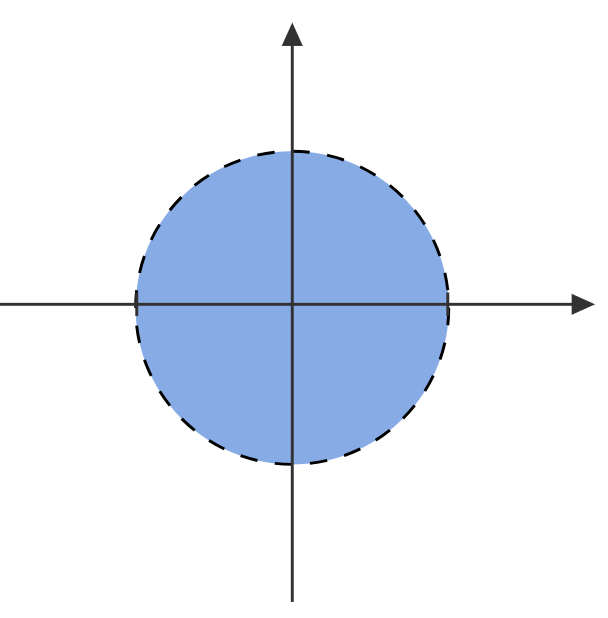
\includegraphics[width=.30\textwidth]{fig191}} \quad
    \subfloat[][\emph{Ball in }$\left( \RR^n, d_1\right)$]
    {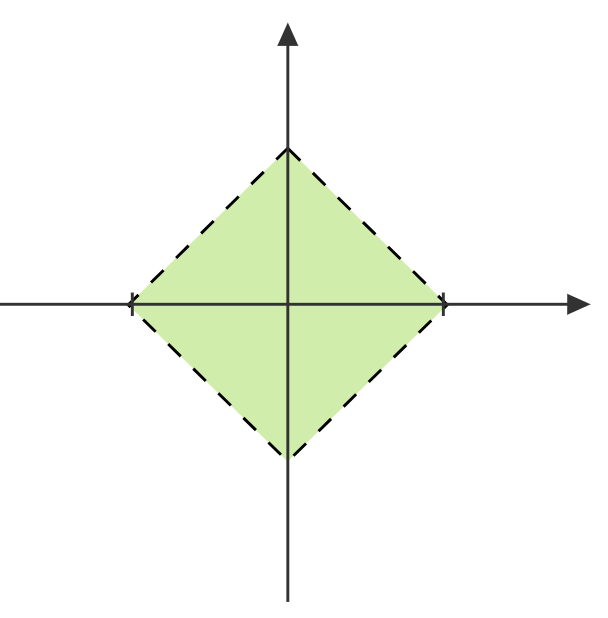
\includegraphics[width=.30\textwidth]{fig192}} \quad
    \subfloat[][\emph{Ball in }$\left( \RR^n, d_\infty\right)$]
    {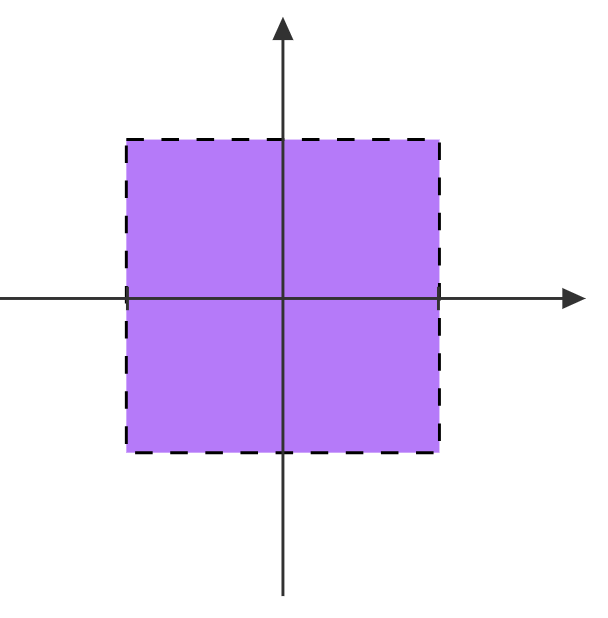
\includegraphics[width=.30\textwidth]{fig193}}
    %\caption*{Funzionamento del quicksort}
    %\label{fig:subfig}
\end{figure}
\end{enumerate}

It is remarkable that these balls are equivalent (we will explain it better in due time). 
\fg{0.4}{fig194}

\newpage

If you generalize to every $p$, you could say that
\fg{0.6}{fig195}

Furthermore, with $(X,d)$ where $d$ is the discrete metric, we have
\begin{equation*}
B_d(x_0,r)=\begin{cases}
    \gr{x_0}, &\text{ if }r\leq 1 \\
    X,&\text{ if }r>1    
\end{cases}
\end{equation*}

Therefore, many possible distances can be introduced on a set. In some cases they lead to the same \emph{structure} but not in genersal. For example, on $X=\Cc^0\left( [a,b] \right)$, $f,g\in X$, we have:
\begin{itemize}
    \item discrete distance (we've got it folks)
    \item $\displaystyle d_1(f,g):=\int_a^b\left| f(x)-g(x) \right|\dx$
    \item $\displaystyle d_\infty(f,g):=\max_{x\in[a,b]}\left| f(x)-g(x) \right|$
\end{itemize}

They are both distances on $\Cc^0\left( [a,b] \right)$ but they lead to different structures:
\fg{0.8}{fig196}

% section recall_on_metric_spaces (end)

\newpage

\section{Topology in metric spaces} % (fold)
\label{sec:topology_in_metric_spaces}

\begin{defn}
Let $(X,d)$ be a metric space and let $A\subset X$. For $x_0\in X$, we say that $x_0$ is:
\begin{enumerate}[(i)]
    \item an \textbf{interior point} of $A$ if
    \begin{equation*}
    \exists r>0\quad\text{s.t.}\quad B(x_0,r)\subset A
    \end{equation*}

    \item an \textbf{exterior point} of $A$ if
    \begin{equation*}
    \exists r>0\quad\text{s.t.}\quad B(x_0,r)\subset A^c:=X\setminus A
    \end{equation*}

    \item a \textbf{boundary point} of $A$ if it is neither interior nor exterior, i.e.
    \begin{equation*}
    B(x_0,r)\cap A\neq\varnothing\quad\text{and}\quad B(x_0,r)\cap A^c\neq\varnothing\quad\forall r>0
    \end{equation*}

    \item an \textbf{adherence point} of $A$ if it is either interior or boundary, i.e.
    \begin{equation*}
    B(x_0,r)\cap A\neq\varnothing\quad\forall r>0
    \end{equation*}

    \item an \textbf{accumulation point} of $A$ if
    \begin{equation*}
    \left( B(x_0,r)\cap A \right)\setminus \gr{x_0}\neq 0
    \end{equation*}

    \item an \textbf{isolated point} of $A$ if
    \begin{equation*}
    x_0\in A\quad\text{and}\quad \exists r>0\quad\text{s.t.}\quad B(x_0,r)\cap A=\gr{x_0}
    \end{equation*}

    \begin{marker}
    By definition, an isolated point cannot be an accumulation point.
    \end{marker}
\end{enumerate}

We also define:
\begin{equation*}
\left.
{\renewcommand*{\arraystretch}{1.5}
\begin{array}{ll}
\overset{o}{A}:=\left\{ x_o\in X\,:\, x_0\text{ is an interior point of }A \right\} &\textbf{interior}\text{ of }A \\
ext(A):=\left\{ x_o\in X\,:\, x_0\text{ is an exterior point of }A \right\} &\textbf{exterior}\text{ of }A \\
\partial A:=\left\{ x_o\in X\,:\, x_0\text{ is a boundary point of }A \right\} &\textbf{boundary}\text{ of }A \\
\overline{A}:=\left\{ x_o\in X\,:\, x_0\text{ is an adherence point of }A \right\} &\textbf{closure}\text{ of }A
\end{array}}
\right.
\end{equation*}
\begin{marker}
The definitions (i)-(ii)-(iii) are mutual disjoint, thus $\overset{o}{A},ext(A),\partial A$ are pairwise disjoint sets (see the property below).
\end{marker}
\end{defn}

\begin{defn}
A set $A\subset X$  is \textbf{open} if $A=\overset{o}{A}$. Similarly, $A$ is \textbf{closed} if $A^c$ is open.
\end{defn}

Let's take a look at some basic properties:
\begin{itemize}
    \item $\overset{o}{A},ext(A),\partial A$ form a partition of $X$
    \item $A$ open iff $A\cap\partial A=\varnothing$
    \item $\overline{A}=\overset{o}{A}\cup\partial A = A\cup\partial A$
    \item $A$ closed iff $A\equiv \overline{A}$
    \item $\overset{o}{A}$ is the largest (w.r.t. the inclusion order) open subset of $A$
    \item $\overline{A}$ is the smallest closed subset of $X$ containing $A$
    \item Let $I$ be a family of indexes (may be uncountable) and $A_i$ be an open set $\forall i\in I$. Then $\displaystyle\bigcup_{i\in I} A_i$ is open.
    \item Let $A_1,...,A_m$ for $m\in\NN$ be a finite number of open sets. Then $\displaystyle\bigcap_{i=1}^m A_i$ is open.
    \begin{home}
    Prove these last two properties.
    \end{home}
    \item Let $I$ be a family of indexes (may be uncountable) and $C_i$ be closed $\forall i\in I$. Then $\displaystyle\bigcap_{i\in I} C_i$ is closed.
    \item Let $C_1,...,C_m$ for $m\in\NN$ be closed. Then $\displaystyle\bigcup_{i=1}^m A_i$ is closed.
    \begin{subtle}
    These last two properties are deduced from the Morgan's laws.
    \end{subtle}
\end{itemize}

% section topology_in_metric_spaces (end)

\section{Limits for sequences} % (fold)
\label{sec:limits_for_sequences}

Let $(X,d)$ metric space, $\left\{ x_n \right\}_{n\in\NN}\subset X$ sequence, $x^*\in X$ point.

\begin{defn}
We say that $x_n\overset{d}\longrightarrow x^*$ as $n\to+\infty$ if
\begin{equation*}
\underbracket[0.2pt]{d(x_n,x^*)\to0}_{\text{limit in real numbers}}\text{ as }n\to+\infty
\end{equation*}
i.e.
\begin{equation*}
\forall\Ec>0\quad\exists \overline{n}=\overline{n}(\Ec)\in\NN\quad\text{s.t.}\quad \underbracket[0.2pt]{d(x_n,x^*)<\Ec}_{\text{or }x_n\in B_d(x^*,\Ec)}\quad \forall n>\overline{n}
\end{equation*}
\end{defn}

\begin{prp}
The limit (it it exists) is unique \underline{in metric space}.
\end{prp}

\begin{home}
Prove it.

\underline{Hint}: assuming by contraddiction that exist $x^*,y^*,x^*\neq y^*$ and then verify the triangular inequality.
\newline
\newline
\newline
\newline
\newline
\newline
(a sketch is in the Cavagnari's slides \texttt{2023-09-18.pdf} on Webeep)
\end{home}

\begin{prp}
If $\left\{ x_n \right\}_{n}$ converges to $x^*$, then any subsequence of $\left\{ x_n \right\}_{n}$ converges and it converges to $x^*$.
\end{prp}

\begin{defn}
A set $A\subset X$ is \textbf{sequentially closed} if for any converging sequence $\left\{ x_n \right\}_{n}\subset A$ its limit $x^*$ belongs to $A$.
\end{defn}

\begin{prp}
$A\subset X$ closed iff $A$ is sequentially closed.
\end{prp}

\begin{home}
Prove it.

\underline{Hint}: for ($\Rightarrow$) use the def. of closed, for ($\Leftarrow$) prove that $A=\overline{A}$ (i.e. $A\subset\overline{A}$ and $\overline{A}\subset A$).
\newline
\newline
\newline
\newline
\newline
\newline
(a solution is in the Cavagnari's slides \texttt{2023-09-18.pdf} on Webeep)
\end{home}

% section limits_for_sequences (end)

\newpage

\section{Closure, Boundedness, Compactness} % (fold)
\label{sec:closure_boundedness_compactness}

Let $(X,d)$ metric space and $E\subset X$ set.

\begin{defn}
The \textbf{diameter} of $E$ is
\begin{equation*}
\text{diam}(E):=\sup_{x,y\in E} d(x,y)\quad\in[0,+\infty]
\end{equation*}
\end{defn}

\begin{defn}
$E$ is \textbf{bounded} if its diameter is finite: $\text{diam}(E)<+\infty$, or equivalently if $\exists R>0$ and $x\in X$ s.t. $E\subset B(x,R)$.
\end{defn}

\begin{defn}
$\left\{ E_i \right\}_{i\in I}\subset\Pc(X)$ is a \textbf{cover/covering} of $E$ if 
\begin{equation*}
E\subset\bigcup_{i=I} E_i
\end{equation*}

A subfamily of $\left\{ E_i \right\}$ which is still a covering for $E$ is called \textbf{subcover/subcovering} of $\left\{ E_i \right\}_{i\in I}$.
\end{defn}

\begin{defn}
$E$ is \textbf{compact} if for any open cover $\left\{ E_i \right\}_{i\in I}$ (i.e. all $E_i$ are open sets) of $E$ there exists a finite subcover (i.e. a finite subset of indexes $J\subset I$ s.t. $E\subset\bigcup_{i\in J}E_i$).
\end{defn}

For example, $E\subset(\RR,d_E)$, $E=(0,1)$ is not compact, indeed if you take $E_n=\left( \nicefrac{1}{n},1 \right)$ then $\left\{ E_n \right\}_{n\in \NN}$ is an open cover for $E$ but it doesn't admit any finite subcover.

\begin{marker}
Let's consider $(X,d)$ with $d$ the discrete metric. We notice that any subset of $X$ is an open set, hence only finite sets (made of a limite number of elements) are compact.
\end{marker}

\begin{thm}
Let $(X,d)$ be a metric space and $E\subset X$ be a compact set. Then $S\subset E$ closed $\Longrightarrow$ $S$ compact.
\end{thm}

\begin{home}
Prove it.
\newline
\newline
\newline
\newline
\newline
\newline
\newline
\newline
(a solution is in the Cavagnari's slides \texttt{2023-09-18.pdf} on Webeep)
\end{home}

\begin{defn}
$E$ is \textbf{sequentially compact} if any sequence $\left\{ x_n \right\}_n\subset E$ admits a convergent subsequence whose limit is in $E$.
\end{defn}

\begin{thm}
Let $(X,d)$ be a metric space and $E\subset X$ be a set. Then:
\begin{enumerate}[(i)]
    \item $E$ is compact $\Longrightarrow$ $E$ closed and bounded
    \item $E$ compact $\Longleftrightarrow$ $E$ is sequentially compact
\end{enumerate}
\end{thm}

\begin{thm}[Heine-Borel]
In $\left( \RR^n,d_E \right)$ (actually any distance), we have $E\subset\RR^n$ compact iff $E$ closed and bounded.
\end{thm}

Its is remarkable that the $\Longleftarrow$ is not true in general, for example it is false in $\infty$-dim. spaces.

% section closure_boundedness_compactness (end)

\newpage

\section{Continuous functions in metric spaces} % (fold)
\label{sec:continuous_functions_in_metric_spaces}

Let $\left( X,d_X \right),\left( Y,d_Y \right)$ be metric spaces and $f:X\to Y$ a function (if $X=\NN$ then $f$ is a sequence).

\begin{marker}
You can have fun proving the followings:
\begin{equation*}
\left.
{\renewcommand*{\arraystretch}{1.5}
\begin{array}{l}
f^{-1}\left( A^c \right)=\left( f^{-1}(A) \right)^c \\
f\left( A_1\cup A_2 \right)=f\left( A_1 \right)\cup f\left( A_2 \right) \\
f\left( A_1\cap A_2 \right)\subset f\left( A_1 \right)\cap f\left( A_2 \right)
\end{array}}
\right.\end{equation*}
\end{marker}

\begin{defn}
$y_0\in Y$ is the \textbf{limit} of $f(x)$ as $x\to x_0\in X$ if
\begin{equation*}
\forall \Ec>0\quad \exists\delta=\delta(\Ec)>0\quad\text{s.t.}\quad \underbracket[0.2pt]{ \underbracket[0.2pt]{0<}_{x\neq x_0}d_X(x,x_0)<\delta\ \Longrightarrow\ d_Y\left( f(x),y_0 \right)<\Ec }_{\displaystyle\text{i.e. }f\left( B_{d_X}\left(x_0,\delta\right)\setminus\left\{ x_0 \right\} \right)\subset B_{d_Y}\left( y_0,\Ec \right)}
\end{equation*}
Then we write $\displaystyle\lim_{x\to x_0}f(x)=y_0$.
\end{defn}

As for sequences, the limit (if exists) is unique.

\begin{defn}
\leavevmode
\begin{enumerate}
    \item $f$ is \textbf{continuous} at $x_0\in X$ if
    \begin{enumerate}[(i)]
        \item $x_0$ is an isolated point

        or

        \item $x_0$ is an accumulation point for $X$ and $f(x_0)=\displaystyle\lim_{x\to x_0} f(x)$
    \end{enumerate}

    \item $f$ is \textbf{sequentially continuous} at $x_0\in X$ if for any sequence $\left\{ x_n \right\}_n\subset X$ s.t. $x_n\overset{d_X}\longrightarrow x_0$, we have that
    \begin{equation*}
    \underbracket[0.2pt]{f\left( x_n \right)\overset{d_Y}\longrightarrow f\left( x_0 \right)\quad\text{as }n\to+\infty}_{\displaystyle\text{i.e. }f\left( x_0 \right)=\lim_{n\to+\infty}f(x_n)\ \text{ i.e. }d_Y\left( f\left( x_n\right),f\left( x_0 \right) \right)\to 0\text{ as }n\to+\infty}
    \end{equation*}
\end{enumerate}
\end{defn}

\begin{thm}
Let $f:\left( X,d_X \right)\to\left( Y,d_Y \right)$ be a function. Then, $f$ is continuous at $x_0\in X$ iff $f$ is sequentially continuous at $x_0$.
\end{thm}

% section continuous_functions_in_metric_spaces (end)

% chapter exercise_session_18_09 (end)























 \cleardoublepage
%!TEX root = ../main.tex

\chapter{}
\thispagestyle{empty} \cleardoublepage
%!TEX root = ../main.tex

\chapter{}
\thispagestyle{empty} \cleardoublepage
%!TEX root = ../main.tex

\chapter{}
\thispagestyle{empty} \cleardoublepage
%!TEX root = ../main.tex

\chapter{}
\thispagestyle{empty} \cleardoublepage
%!TEX root = ../main.tex

\chapter{}
\thispagestyle{empty} \cleardoublepage
%!TEX root = ../main.tex

\chapter{}
\thispagestyle{empty} \cleardoublepage
%!TEX root = ../main.tex

\chapter{}
\thispagestyle{empty} \cleardoublepage
%!TEX root = ../main.tex

\chapter{}
\thispagestyle{empty} \cleardoublepage
%!TEX root = ../main.tex

\chapter{}
\thispagestyle{empty} \cleardoublepage

\end{document}